+++Motivate motivate motivate+++\\
Nonlinear evolution equations ubiquitous across the sciences. These typically take the form
$$ \dot{x}(t) = F\left(x(t)\right)$$ where $x\in \mathbf{R}^n, F\in C^r(\mathbf{R}^n,\mathbf{R}^n)$. We will be interested in systems that occur on different timescales, known as fast-slow systems. These occur naturally in physics, neuroscience and many other biological scenarios +++ Van der Pol, FitzHugh-Nagumo, other bio ref?+++. Models of such systems can be written generally in the form given below.

\begin{align}
\begin{cases}
x' &=\frac{dx}{dt}= f(x,y,\epsilon),\\
y' &= \frac{dy}{dt}= \epsilon g(x,y,  \epsilon),
\end{cases}\label{FastS}
\end{align} 
Here, $x \in \R^n, y \in R^m, m,n \geq 1$ and $f,g$ are sufficiently smooth. The separation in timescales is governed by $0<\epsilon \ll 1$, known as the timescale separation parameter. Some systems also act on more than two timescales, in which case there is more than one timescale separation parameter.  In the system above, note that the change in $x$ is $O(1)$, whilst it is $O(\epsilon)$ in $y$. As $\epsilon$ is very small, this means that the change in $x$ is much faster than that of $y$. If we slow down time with the transformation $\tau = \epsilon t$, the system becomes  
\begin{align}
	\begin{cases}
	\epsilon \dot{x} &= \epsilon \frac{dx}{d\tau} = f(x,y,\lambda, \epsilon),\\
	\dot{y} & = \frac{dy}{d \tau} =  g( x,y, \lambda, \epsilon),
	\end{cases}\label{SlowS}
\end{align} 
Represented like this, $\dot{x} = O(\frac{1}{\epsilon})$ whilst $\dot{y} = O(1)$.  The time scale given by $\tau$ is said to be slow so (\ref{SlowS}) is the \emph{slow system} while (\ref{FastS}) is the \emph{fast system}.


\begin{figure}[]
	%\includegraphics[]}
	\caption{Examples of fast-slow systems in nature (neuron,ECG etc. )}
	\label{fig:nature}
\end{figure} 


Throughout what follows, the motivating example will be the Van der Pol equation. The Van der Pol oscillator is a well-studied second order ODE that is used to model a variety of physical and biological phenomena. It was developed by the Dutch physicist and electrical engineer Balthasar Van der Pol, who conducted research on electrical circuits. This equation can be scaled so that it becomes a fast-slow system of the form shown in Equation\ref{FastS} after a change of variables.

\subsection{Derivation of the Van der Pol Fast-Slow System}

The Van der Pol Oscillator describes the evolution of the position coordinate \(x(t)\) according to the following the ODE:
\begin{equation} \label{eq:vdP}
\ddot{x}(t)-\mu\left(1-x^2(t)\right)\dot{x}(t)+x(t)=0,
\end{equation}
where \(\mu \gg 1\) is a scalar constant. \\

In order to analyse systems (\ref{FastS}) and (\ref{SlowS}) using Geometric Singular Pertubation Theory (GSPT), the singular limit $\epsilon \to 0$ is considered:

\begin{align} \label{FastS0}
\begin{cases}
x' &=\frac{dx}{dt}= f(x,y,\lambda, \epsilon)\\
y' &= 0,
\end{cases}
\end{align}
which is called the layer problem, and
\begin{align}\label{SlowS0}
\begin{cases}
0 &= \epsilon \frac{dx}{d \tau} = f(x,y,\lambda, 0)\\
\dot{y} & = \frac{dy}{d \tau} =  g( x,y, \lambda,0),
\end{cases}
\end{align}
called the reduced system.\\


In order to analyse systems (\ref{FastS}) and (\ref{SlowS}) using Geometric Singular Perturbation Theory (GSPT), the singular limit $\epsilon \to 0$ is considered:

\begin{align} \label{FastS0}
\begin{cases}
x' &=\frac{dx}{dt}= f(x,y,\lambda, \epsilon)\\
y' &= 0,
\end{cases}
\end{align}
which is called the layer problem, and
\begin{align}\label{SlowS0}
\begin{cases}
0 &= \epsilon \frac{dx}{d \tau} = f(x,y,\lambda, 0)\\
\dot{y} & = \frac{dy}{d \tau} =  g( x,y, \lambda,0),
\end{cases}
\end{align}
called the reduced system.\\

Now considering Equation \ref{SlowS0}, we can write $f(x,y,\lambda, 0)=0$. Then we are able to define the critical manifold as:,
\begin{align} \label{CriticalS}
S= \left\{ (x,y) : f(x,y,\lambda, 0)=0 \right \},
\end{align}
where, by definition of $S$, the points $(x,y) \in S$ are equilibria of (\ref{FastS0}). Before we continue, it is useful to have a visual interpretation of these flows,
\begin{figure}[h!]\centering

	\begin{subfigure}[t]{0.45\textwidth}
		\centering
		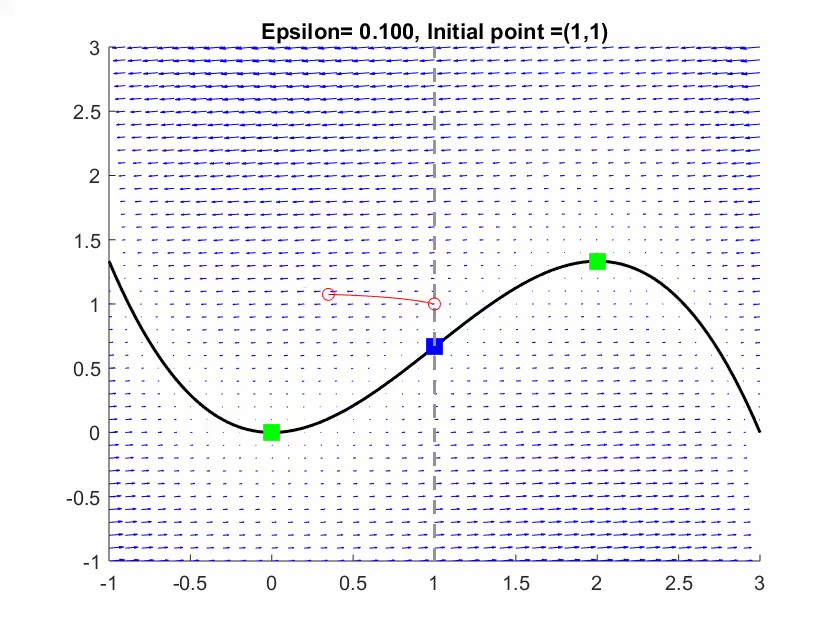
\includegraphics[width=.8\linewidth]{vdPhopf-Moment-1.jpg}
		\caption{The initial flow within the system starting at $ (x,y)=(1,1) $.}
	\end{subfigure}
	\hfill
	\begin{subfigure}[t]{0.45\textwidth}
		\centering
		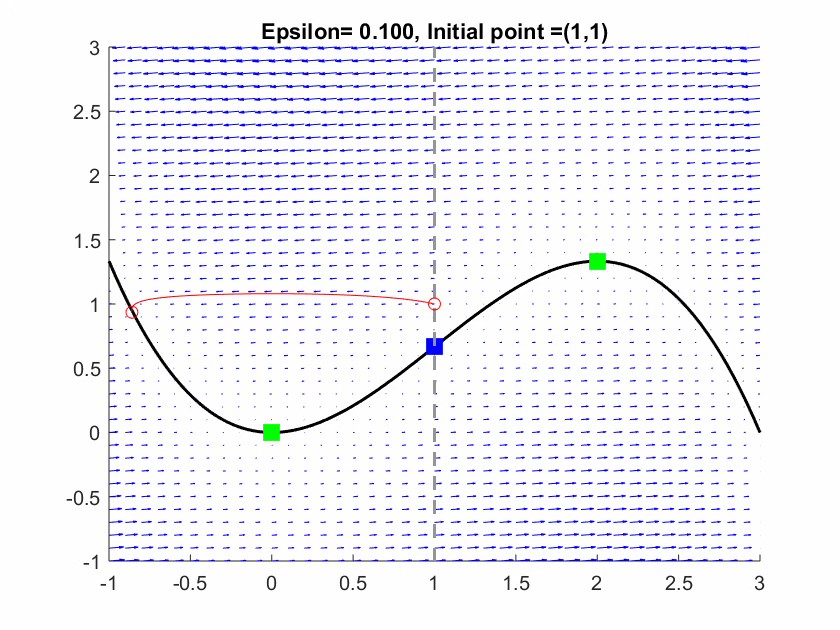
\includegraphics[width=.8\linewidth]{vdPhopf-Moment-2.jpg}
		\caption{The flow as it hits the slow manifold.}
	\end{subfigure}

	\vspace{1cm}
	\begin{subfigure}[t]{0.45\textwidth}
		\centering
		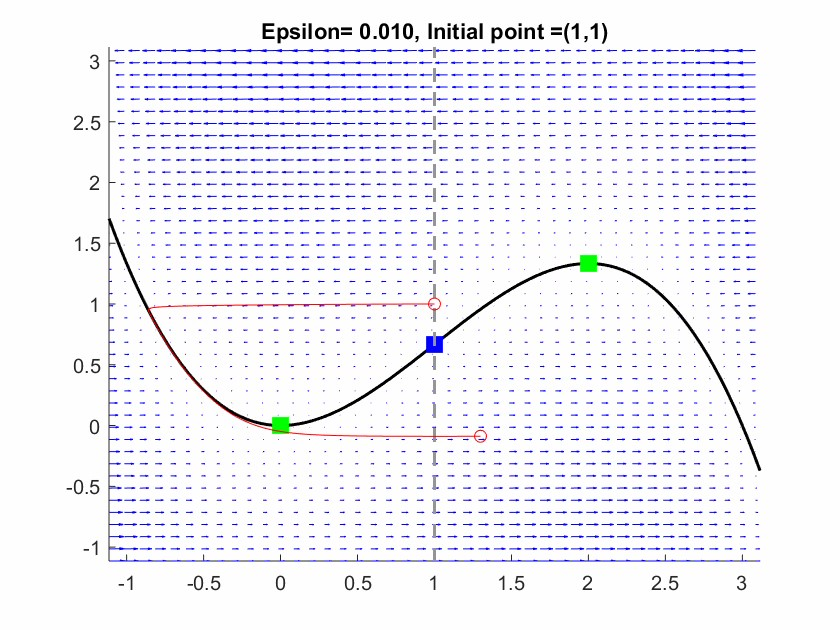
\includegraphics[width=.8\linewidth]{vdp-jump1}
		\caption{The flow as it intersects with the fold point and begins the jump.}
	\end{subfigure}
	\hfill
	\begin{subfigure}[t]{0.45\textwidth}\centering
		% just an empty subfigure to shift C below A
		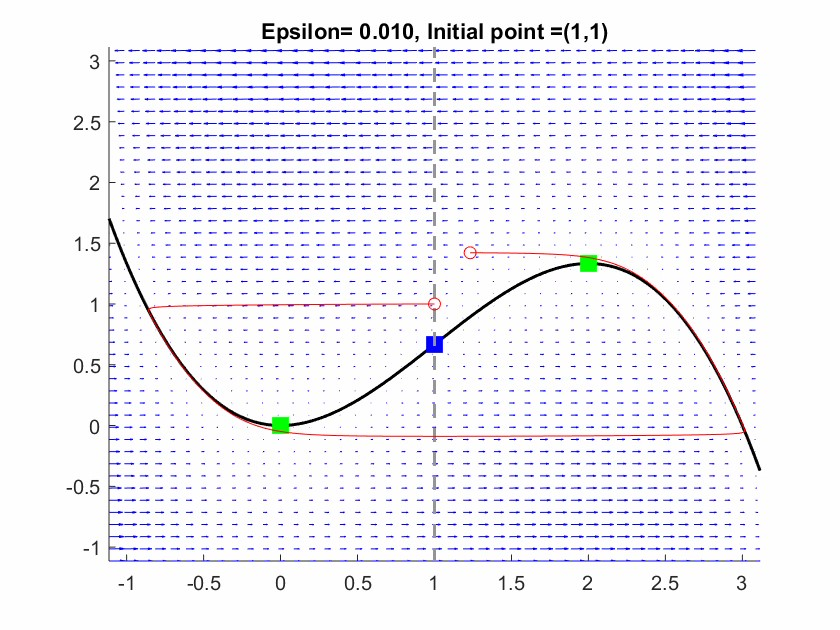
\includegraphics[width=.8\linewidth]{vdp-jump2}
		\caption{The second jump before continuing in a periodic fashion.}
	\end{subfigure}
	\caption{Flows in the \vdp system.}
	\label{fig: vdp flow diagram}
\end{figure}\newline
where we can see that the flows will travel towards our fold point, following the relevant branches. It is worth noting that our flow does not meet the fold point exactly, although this is an `error', it does not directly effect our simulations - as is discussed in Section \ref{sec:matlab-stuff}.
